\documentclass[12pt,letterpaper]{article}
\usepackage{preamble}
\usepackage[brazil]{babel}
\usepackage[utf8]{inputenc}
\usepackage{enumitem}

%%%%%%%%%%%%%%%%%%%%%%%%%%%%%%%%%%%%%%%%%%
%%%% Edit These for yourself
%%%%%%%%%%%%%%%%%%%%%%%%%%%%%%%%%%%%%%%%%%
\newcommand\course{IA753}
\newcommand\hwnumber{1}
\newcommand\userID{Heitor S. Fernandes - RA: 074096}

\begin{document}
\centerline{\textbf{\Large Trabalho Computacional \hwnumber}}

\centerline{\text{ Linguagem utilizada: Python }}

\section*{Questão 1. Análise espectral do ECG}
\begin{enumerate}[label=(\alph*)]  %,leftmargin=!,labelindent=5pt]
    \item O sinal foi carregado a partir do arquivo \emph{signal.txt}. A frequência de amostragem ${f_s = 500 Hz}$ foi utilizada para calcular o tamanho do passo temporal: ${dt = 1/f_s = 0.002}$ segundos . A partir de ${dt}$ e do número de amostras ${N = 1000}$, foi criado um vetor tempo, indo de 0.000 a 19.998 segundos.
        \begin{figure}[H]
            \centering
            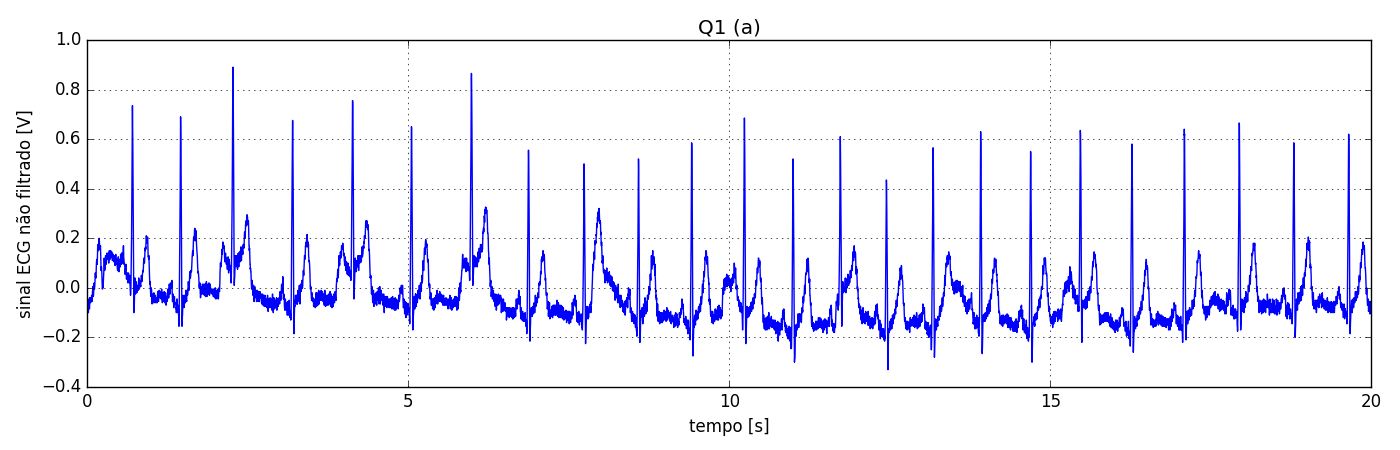
\includegraphics[width=15cm]{TC1/images/Q1_a_sinal_nfilt.png}
            \caption{Sinal de ECG em função do tempo.}
            \label{fig:1}
        \end{figure}

    \item
    Foi utilizado o comando \lstinline{np.fft.rfft} para obter a FFT do sinal. Outra maneira seria utilizar a FFT complexa (\lstinline{np.fft.fft}) e utilizar a apenas a parte real da resposta. O comando \lstinline{np.fft.rfftfreq} fornece as frequências de amostragem, porém em unidade adimensional. Para calibrar o eixo das abscissas em Hertz foi calculada a resolução espectral como o inverso do tempo se amostragem, isto é, ${df = {1/(dt*N)} = 0.05 Hz}$, e utilizado o número de amostras $N$.
    
    $${f_{Hz} = f_{adim}*df*N = {f_{adim} \over {dt*N}} *N = {f_{adim} \over dt}}$$
    
        \begin{figure}[H]
            \centering
            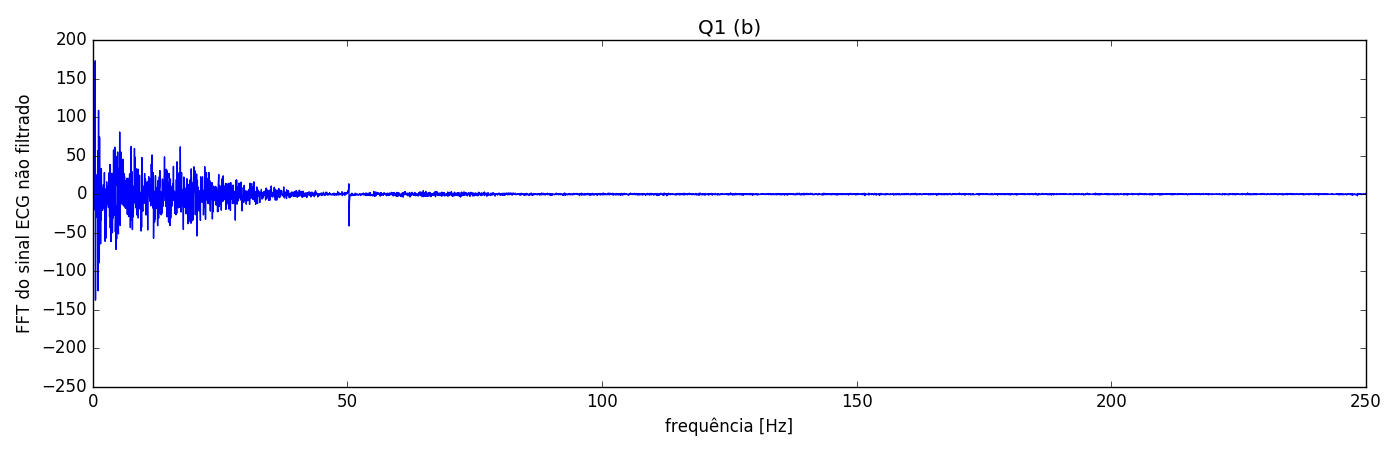
\includegraphics[width=15cm]{TC1/images/Q1_b_espectro_nfilt.png}
            \caption{Espectro do sinal de ECG.}
            \label{fig:2}
        \end{figure}
        
    \item
    O espectro possui componentes próximas a 50Hz, possivelmente devido à interferência da rede elétrica do local. São observadas, também, componentes em baixas frequências que podem estar relacionadas à respiração ou outros movimentos do indivíduo durante a aquisição do sinal e componentes em alta frequência, que podem estar relacionadas à detecção de sinais de EMG e ruídos causados pelos fios e pela interface entre a pele e os eletrodos.
    
\end{enumerate}

\section*{Questão 2. Filtragem digital}
Para criar os filtros foram utilizadas funções da biblioteca \lstinline{scipy.signal}.
\begin{enumerate}[label=(\alph*)]  %,leftmargin=!,labelindent=5pt]
    \item Filtro passa-baixas.
    
    (a.1)(a.2) O filtro passa-baixas foi projetado com as seguintes restrições: atenuação em 50Hz de 40dB (ou seja, faixa de rejeição iniciando em 50Hz), ordem máxima do filtro igual a 10 (para evitar instabilidade do filtro) e atenuação máxima de 3dB na faixa de passagem. Com estas restrições a faixa de passagem foi um resultado do projeto do filtro. Iterativamente, foi utilizada a função \lstinline{buttord} fixando-se a frequência da faixa de rejeição ($f_{stop}$) em 50Hz, a atenuação na faixa de passagem em 3dB e a atenuação na faixa de rejeição em 40dB. Desta maneira a frequência de corte máxima para obter um filtro de ordem máxima igual a 10 foi de $f_{pass} = 32Hz$.
    
    Então, foi utilizada a função \lstinline{butter} para gerar o filtro ButterWorth passa-baixas de ordem 10 e frequência de corte de 32Hz.
    
    (a.3) Função de transferência do filtro passa-baixas:
    
    $${Y(z) \over X(z)} = H(z) =
        {
        { \sum_{k=0}^{10}{b_k z^{-k}} }
        \over
        { \sum_{l=1}^{10}{a_l z^{-l}} }
        }
    $$
    
    Com os valores dos coeficientes $b_k$ e $a_l$ abaixo:
    
    \begin{table}
    \centering
    \begin{tabular}{lllll}
        $b_{0}$ & 3.39e-08 & \space & $a_{0}$ & 1.00 \\ 
        $b_{1}$ & 3.39e-07 & \space & $a_{1}$ & -7.43 \\ 
        $b_{2}$ & 1.53e-06 & \space & $a_{2}$ & 25.10 \\ 
        $b_{3}$ & 4.07e-06 & \space & $a_{3}$ & -50.73 \\ 
        $b_{4}$ & 7.12e-06 & \space & $a_{4}$ & 67.86 \\ 
        $b_{5}$ & 8.54e-06 & \space & $a_{5}$ & -62.73 \\ 
        $b_{6}$ & 7.12e-06 & \space & $a_{6}$ & 40.57 \\ 
        $b_{7}$ & 4.07e-06 & \space & $a_{7}$ & -18.12 \\ 
        $b_{8}$ & 1.53e-06 & \space & $a_{8}$ & 5.34 \\ 
        $b_{9}$ & 3.39e-07 & \space & $a_{9}$ & -0.94 \\ 
    \end{tabular}
    \end{table}
    
    Abaixo estão apresentados o espectro do sinal após o filtro passa-baixas e um comparativo do sinal antes e depois do filtro.
    
    
    
\newpage
    (a.4) Caso a frequência de corte seja maior, as componentes perto de $50Hz$ serão menos atenuadas e para frequências de corte ainda menores que $32Hz$, aumenta a quantidade de informação que está sendo atenuada mas que poderia ser desejada para caracterizar o sinal de ECG.
    
    Abaixo, mostra-se o sinal filtrado em três frequências de corte: $22Hz$, $32Hz$ (do filtro original) e $42Hz$.

        \begin{figure}[H]
            \centering
            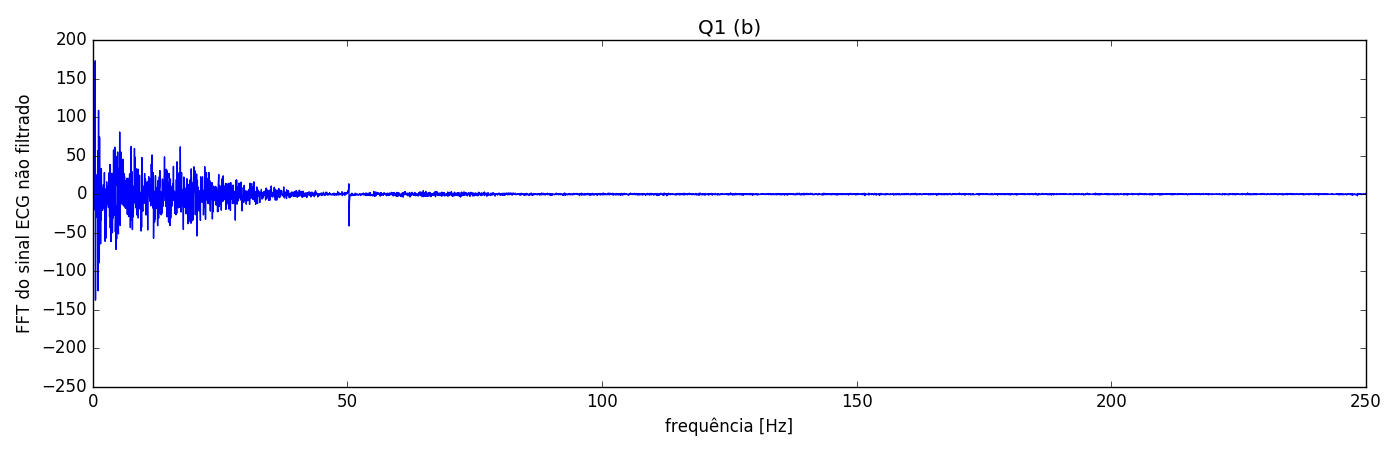
\includegraphics[width=15cm]{TC1/images/Q1_b_espectro_nfilt.png}
            \caption{Espectro do sinal de ECG.}
            \label{fig:3}
        \end{figure}


     \item  Filtro passa-altas.
    \begin{enumerate}[label=(b.\arabic*)]
        \item Frequência de corte.
        \item Ordem do filtro.
        \item Sinal filtrado' vs não filtrado.
        \item Variar frequências de corte.
    \end{enumerate}
    \item Filtro Notch.
    \item Combinação de filtros.
\end{enumerate}


\section*{Questão 3. Estimar frequência instantânea.}
\begin{enumerate}[label=(\alph*)]  %,leftmargin=!,labelindent=5pt]
    \item Identificar os picos no ECG.
    \item Criar trem de impulsos.
    \item Janelamento.
\end{enumerate}

\end{document}
